\documentclass[11pt, oneside]{article}   	% use "amsart" instead of "article" for AMSLaTeX format
\usepackage{geometry}                		% See geometry.pdf to learn the layout options. There are lots.
\geometry{letterpaper}                   		% ... or a4paper or a5paper or ... 
%\geometry{landscape}                		% Activate for for rotated page geometry
%\usepackage[parfill]{parskip}    		% Activate to begin paragraphs with an empty line rather than an indent
\usepackage{graphicx}				% Use pdf, png, jpg, or eps� with pdflatex; use eps in DVI mode
								% TeX will automatically convert eps --> pdf in pdflatex		
\usepackage{amssymb}
\usepackage{amsmath}
\usepackage{parskip}
\usepackage{color}
\usepackage{hyperref}

\title{Oscillations using complex numbers}
%\author{The Author}
%\section{}
%\subsection*{}
\date{}							% Activate to display a given date or no date

\graphicspath{{/Users/telliott_admin/Dropbox/Tex/png/}}
% \begin{center} 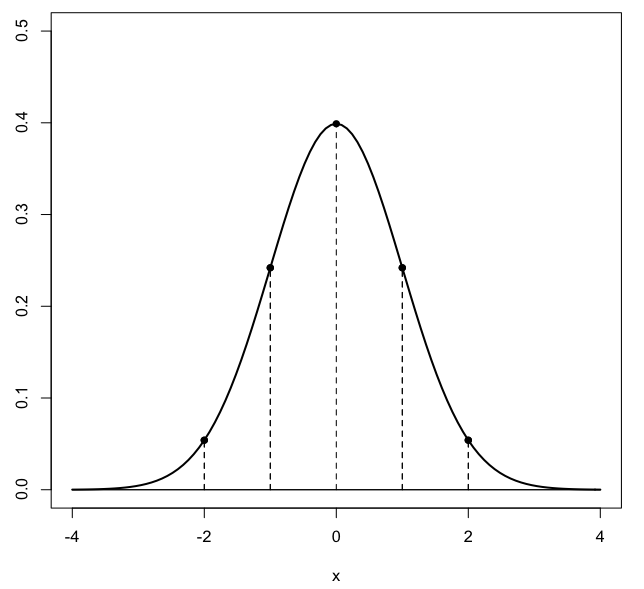
\includegraphics [scale=0.4] {gauss3.png} \end{center}
\begin{document}
\maketitle
\Large
I'm working through the derivation of equations for oscillation, damped oscillation, and driven oscillation, starting with Prof. Shankar's approach in the online course (Lecture 18).

To begin with, consider the equation for a mass on a spring (on a frictionless table):
\[ F = - kx \]
we don't need vectors for this since we are working in one dimension.  By experiment, we find that the force is proportional to the displacement and directed toward the equilibrium position.  Newton's Law says that $F=ma$ so
\[ m \ddot{x} = - kx \]
\[ \ddot{x} + \frac{k}{m} x = 0 \]
This equation is easy to solve, one possibility is
\[ x(t) = A \cos \omega t \]
\[ \ddot{x}(t) = - \omega^2 A \cos \omega t \]
so that
\[ (- \omega^2 + \frac{k}{m}) A \cos \omega t = 0 \]
\[ \frac{k}{m} = \omega^2 \]
\[ \omega = \sqrt{k/m} \]
Observe that $A$ can be anything we want.  In particular, it corresponds to the maximum amplitude of the oscillation, determined by how far we pull out the mass to start things off.

In contrast, $\omega$ is determined by the characteristics of the spring, and inversely proportional to the mass.  It is also related to the frequency of oscillation.  If $T$ is the time period for one complete oscillation, then $\omega T = 2 \pi$, or if $f$ is the frequency of oscillation, then $\omega = 2 \pi f$.

Finally, this solution assumes that $v_0 = 0$
\[ \dot{x}(t) = - \omega A \sin \omega t \]
\[ \dot{x}(0) = - \omega A \sin \omega 0 = 0 \]
That is more restrictive than necessary.  We can deal with this in various ways, one is to add a term containing the sine
\[ x(t) =  A \cos \omega t + B \sin \omega t\]
\[ \dot{x}(t) =  - \omega A \sin \omega t + B \cos \omega t\]
\[ \dot{x}(0) = B = v_0 \]
Another way is to add a phase term to the angle, which doesn't change the derivatives
\[ x(t) =  A \cos \omega t + \phi \]
\[ \dot{x}(t) = - \omega A \sin \omega t + \phi \]
\[ \dot{x}(0) = v_0 = - \omega A \sin \phi \]

It is interesting to see why these amount to the same thing.  Recall
\[ \cos \omega t + \phi = \cos \omega t \cos \phi - \sin \omega t \sin \phi \]
But $\phi$ is a constant so if $-B = \sin \phi$ and $A = \cos \phi$
\[ \cos \omega t + \phi = A \cos \omega t + B \sin \omega t \]

Another thing Prof. Shankar does is to verify the Conservation of Energy
\[ x(t) = A \cos \omega t \]
\[ v = \dot{x} = - \omega A \sin \omega t \]
\[ E = \frac{1}{2}mv^2 + \frac{1}{2} kx^2 \]
\[ = \frac{1}{2}m \omega^2 A^2 \sin^2 \omega t + \frac{1}{2} k A^2 \cos \omega t \]
But $\omega^2 = k/m$ so
\[ = \frac{1}{2}k A^2 \sin^2 \omega t + \frac{1}{2} k A^2 \cos \omega t \]
\[ E = \frac{1}{2}k A^2 \]

\subsection*{friction}
Next, we consider the same system but with friction.  Now the equation becomes
\[ m\ddot{x} + b \dot{x} + k x = 0 \]
\[ \ddot{x} + \gamma \dot{x} + \frac{k}{m} x = 0 \]
(where $\gamma = b/m$).  Another substitution for $\omega^2 = k/m$ (and now we will call it $\omega_0$ because there will be more of them later
\[ \ddot{x} + \gamma \dot{x} + \omega_0{}^2 x = 0 \]
Because of the term containing $\dot{x}$, the trig functions won't work so easily any more.  Let's guess that the solution is an exponential
\[ x = A e^{\alpha t} \]
\[ \dot{x} = \alpha A e^{\alpha t} \]
\[ \ddot{x} = \alpha^2 A e^{\alpha t} \]
Substituting, we obtain
\[ (\alpha^2 + \alpha \gamma + \omega_0{}^2 ) A e^{\alpha t} = 0 \]
For this to be zero, the term in parentheses must be equal to zero.  
\[ \alpha^2 + \alpha \gamma + \omega_0{}^2 = 0 \]
From the quadratic equation, then, we have two solutions
\[ \alpha = -\frac{\gamma}{2} \pm \sqrt{(\frac{\gamma}{2})^2 - \omega_0{}^2} \]
These solutions may be real (for $(\gamma/2)^2 \ge \omega_0{}^2$), or not.  If they are real, observe that $\alpha < 0$ (even if $\omega_0{}^2 = 0$).  So we can write
\[ x(t) = A e^{-|\alpha|t} \]
and that negative exponential is good, since it means the motion damps out with time.  We don't want a positive exponential, because that would not correspond to what we observe the system to do.

Going back to the two solutions, we will add them together like this
\[ x(t) = A e^{-|\alpha_+|t} + B e^{-|\alpha_-|t} \]
We justify this by the principle of superposition.  Namely, since the two solutions don't interact, when we take derivatives, the left and right-hand sides will just be the sums of what we obtained before.

With 
\[ \alpha_+ = -\frac{\gamma}{2} + \sqrt{(\frac{\gamma}{2})^2 - \omega_0{}^2} \]
\[ \alpha_- = -\frac{\gamma}{2} - \sqrt{(\frac{\gamma}{2})^2 - \omega_0{}^2} \]
At $t=0$
\[ x(0) = A  + B \]
\[ \dot{x}(0) = v_0 = - |\alpha_+| A - |\alpha_-| B \]
Two equations in two unknowns, which we can solve for $A$ and $B$ given $x_0$ and $v_0$ (and $\omega_0$ and $\gamma$).

\subsection*{complex solutions}
Life is not that simple, however.  There are additional solutions to this problem, corresponding to the situation where $\omega_0{}^2 > (\gamma/2)^2$.  In that case, switch the sign of what's under the radical and pull out $\sqrt{-1} = i$:
\[ \alpha = -\frac{\gamma}{2} \pm i\sqrt{(\omega_0{}^2 - \frac{\gamma}{2})^2} \]
Call this 
\[ \omega' = \sqrt{(\omega_0{}^2 - \frac{\gamma}{2})^2} \]
so 
\[ \alpha = -\frac{\gamma}{2} \pm i\omega' \]
Our previous solution was
\[ x(t) = A e^{-|\alpha_+|t} + B e^{-|\alpha_-|t} \]
Now we have
\[ x(t) = A e^{(-\gamma/2 + i\omega')t} + B e^{(-\gamma/2 - i\omega')t} \]
\[ x(t) = A e^{-\gamma/2 t} e^{i\omega't} + B e^{-\gamma/2 t} e^{-i\omega't} \]
Now, you may see a complication with this.  Namely, $x$ \emph{is real}.  How can we have an equation with $i$ in it?  The answer is that the two terms must be each other's complex conjugate.  We are part of the way there, with the minus sign on the imaginary exponent in the second term.  What remains is that
\[ B = A^* \]
Any number plus its complex conjugate is completely real, and is equal to  twice the value of the real part of the number.
\[ (a + bi) + (a - bi) = 2a \]
\[ z + z^* = 2 Re(z) = 2 |z| \]
So
\[ x(t) = A e^{-\gamma/2 t} e^{i\omega't} + A^* e^{-\gamma/2 t} e^{-i\omega't} \]
\[ = e^{-\gamma/2 t} (A e^{i\omega't} + A^* e^{-i\omega't} )  \]
Now let
\[ A = |A|e^{i\phi} \]
\[ A^* = |A|e^{-i\phi} \]
So 
\[ x(t) = e^{-\gamma/2 t} (|A| e^{i\phi} e^{i\omega't} + |A|e^{-i\phi} e^{-i\omega't} )  \]
\[ = |A| e^{-\gamma/2 t} ( e^{i(\omega' t - \phi)} + e^{-i(\omega't - \phi)} )  \]

Recall that
\[ 2 \cos \theta = e^{i \theta} + e^{-i \theta} \]
If
\[ C = 2 |A| \]
then
\[ x(t) = C e^{-\gamma/2 t} \cos (\omega' t - \phi)   \]
Addition of a phase term will not change the fact that this is a solution.  And it doesn't really matter that we have $-\phi$.  Another solution is
\[ x(t) = C e^{-\gamma/2 t} \cos (\omega' t + \phi)   \]

This is a solution with friction, but without a driving force.  It is called $x_c$ for \emph{complementary}.

\subsection*{driven oscillator}
You may suspect that we are not done yet, and that would be correct!

For this last part, consider
\[ \ddot{x} + \gamma \dot{x} + \frac{k}{m} x = \frac{F_0}{m} \cos \omega t \]
Rather than solve this, we instead solve
\[ \ddot{z} + \gamma \dot{z} + \frac{k}{m} z = \frac{F_0}{m} e^{i \omega t} \]
where $z$ is a complex number and so is the right-hand side.  Guess a solution
\[ z = z_0 e^{i\omega t} \]
Then $\dot{z}$ gives $i \omega$ and $\ddot{z}$ gives $- \omega^2$ and we obtain
\[ (-\omega^2 + i \omega \gamma + \omega_0^2) \ z_0 e^{i\omega t} = \frac{F_0}{m} e^{i\omega t} \]
Call
\[ I(\omega) = I = (\omega_0^2 - \omega^2) + i \omega \gamma \]
The modulus or length of $I$ is
\[ |I| = \sqrt{\omega_0^2 - \omega^2)^2 + \gamma^2 \omega^2} \]
\[ I = |I|  e^{i\phi} \]
\[ \phi = \tan^{-1} \frac{\omega \gamma}{\omega_0^2 - \omega^2} \]
so then we have
\[ z(t) = I z_0 e^{i\omega t} = \frac{F_0}{m} e^{i\omega t} \]
\[ I z_0 e^{i\omega t} = \frac{F_0}{m} e^{i\omega t} \]
\[ I z_0  = \frac{F_0}{m}  \]

Finally,
\[ z(t) = F_0/m \ \frac{e^{i\omega t}}{ |I| e^{i \phi} }  \]
\[ = \frac{F_0/m}{|I|} \ e^{i (\omega t - \phi)} \]
We take the real part of this as our solution
\[ x(t) = \frac{F_0/m}{|I|} \  \cos(\omega t - \phi) \]
We add to it the solution found above $x_c$, which allows us to fit the solution to initial parameters.  The latest solution is called $x_p$ for $x$ \emph{particular}.
\[ x_p = \frac{F_0/m}{|I|} \  \cos(\omega t - \phi) \]
\[ x(t) = x_p + x_c \]
\[ = \frac{F_0/m}{|I|} \  \cos(\omega t - \phi) +  C e^{-\gamma/2 t} \cos ( \omega' t + \phi)   \]

\end{document}  